\subsection{Generación de instancias aleatorias}
El método de generación de instancias aleatorias se basa en un sistema de instancias sinteticas
que se generan a partir de un conjunto de parámetros de entrada. En el siguiente paper \cite{pbrandimarte}
se define una tabla con diferentes rangos de valores para cada parámetro en cada conjunto de
tamaños de instancias. En nuestro caso, se va a utilizar tres conjuntos de tamaños de instancias
represantados en la siguiente tabla.

\begin{table}[ht]
    \centering
    \begin{tabular}[t]{|l|ccc|}
        \hline
                  & Ins. Pequeña & Ins. Medianas & Ins. Grandes \\
        \hline
        Min. num Trabajos    & 3    & 1.122    & 0.754 \\
        Max. num Trabajos    & 5    & 1.122    & 0.754 \\
        Min. num Operaciones & 2    & 1.122    & 0.754 \\
        Max. num Operaciones & 5    & 1.122    & 0.754 \\
        Min. num Maquinas    & 2    & 1.122    & 0.754 \\
        Max. num Maquinas    & 4    & 1.122    & 0.754 \\
        \hline
    \end{tabular}
    \caption{Conjuntos de tamaños de instancias}
\end{table}

En este caso se va a almacenarlas las instancias una vez generadas para poder asegurar la reproducibilidad 
de los resultados, esto adicionalmente implica otros veneficios como el ahorro de tiempo de procesamiento
a la hora de entrar el modelo que se vera altamente beneficiado cuando en pasos posteriores se calcule
las rutas optimas de frabicación de las instancias. Estas conforman nuestro conjunto de datos de 
entrenamiento, de los cuales extraeremos una pequeña parte por cada grupo de instancias para formar
diferentes conjuntos de validacion. 

\subsection{Modelos de programación matemático}
Los modelos de programación matemática son una herramienta muy poderosa para resolver problemas
de optimización, en este caso se va a utilizar una librería de código abierto llamada OR-Tools 
\cite{ortools} que esta desarrollada por Google y es utilizada para resolver problemas de optimización 
combinatoria. La libreria proporciona algoritmos para resolver una amplia variedad de problemas 
de programación matemática, como problemas de programación lineal, programación entera mixta, 
programación de enteros, y otros problemas de optimización combinatoria.\medskip 

Dentro de la librería se encuentra un modulo llamado \textbf{CP-SAT} que es un modulo de programación
de restricciones que utiliza el algoritmo de búsqueda de satisfacción de restricciones (CS) para resolver
problemas de programación de tareas. Este modulo es el que se va a utilizar para resolver el problema y
dentro de la documentación \cite{ortools-jobshop} de la librería se encuentra un ejemplo de como 
aplicarlo de forma sencilla. La entrada de OR-Tools es una lista de tareas, donde cada tarea contiene
una lista de máquinas que pueden realizar la operacion junto con el tiempo de procesamiento.\medskip

\begin{lstlisting}
    jobs_data = [                   
        [(0, 3), (1, 2), (2, 2)],   # Job0
        [(0, 2), (2, 1), (1, 4)],   # Job1
        [(1, 4), (2, 3)]            # Job2
    ]
   
    proccess_jobs(jobs_data)

    Output:
    Machine 0: [0,3] [3,5]
    Machine 1: [0,4] [4,6] [7,11]
    Machine 2: [5,6] [6,8] [8,11]
\end{lstlisting}

Este resultado muestra una configuracion optima de frabricación, de la que se pueden extraer
adicionalmente los tiempos de inicio y fin de cada operación, una representacion en forma de
diagrama de Gantt y el makespan de la configuración. El makespan es el tiempo total que se 
tarda en completar todas las operaciones de la configuración, y es el valor que se va a utilizar
para evaluar la precision de los modelos de deep learning. Con este valor ya seriamos capaces
de comformar los diferentes sets de validación, ya que para esta no es necesario como tal ningun
dato adicional. 

\subsection{Entrenamiento del modelo de deep learning}
\subsubsection{Arquitectura del modelo basico}
La arquitectura del modelo de deep learning se forma a partir de la combinación de tres 
modelos basados en redes neuronales de grafos que forman un unico modelo que es capaz 
de adaptarse a los diferentes tipos de instancias que tenga que predecir. Normalmente en el
ensemble learning se utiliza diferentes tecnicas como la votación o la media de los resultados
para elegir las diferentes acciones que se van a tomar, esto es debido a que en ese tipo de problemas
no suele haber una unica solución correcta o a que no existe un criterio que permita 
elegir una solución sobre otra. En nuestro caso, debido al claro objetivo que es reducir 
el makespan, se va a utilizar la solución que tenga el menor makespan de entre las tres 
generadas por los modelos. Los tres modelos que se van a seleccionar son aquellos tres 
que mejor resultado hayan dado en la fase de validación.\medskip

A continuación, se puede ver como esta definido el modelo basado en redes neuronales de grafos.
Para este caso se ha estan utilizando capas convolucionales GATv2Conv que son específicas para
el procesamiento de aristas dentro de grafos. Estas capas convolucionales pertencen a la librería
de Pytorch Geometric \cite{pytorch-geometric} que es una librería de código abierto que proporciona
implementaciones de algoritmos de aprendizaje profundo sobre grafos. 

\begin{figure}[ht]
    \centering
    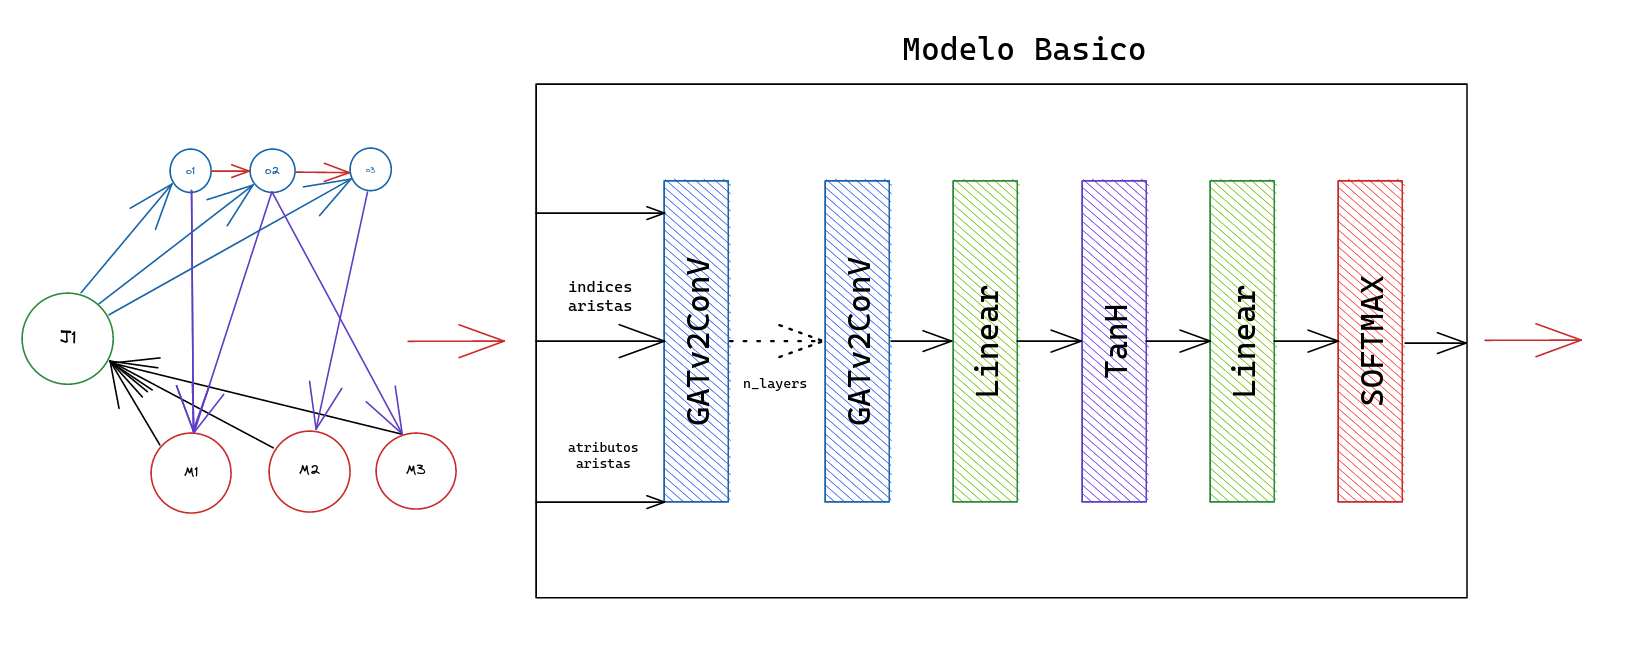
\includegraphics[scale=0.25]{normalmodel.png}
    \caption{Modelo basado en redes neuronales de grafos}
    \label{fig:basicmodel}
\end{figure}

Esta versión del modelo funciona como un agente de RL que recibe como entrada un grafo que representa
un estado del problema, y como salida devuelve la acción que debe tomar para avanzar al siguiente estado.
Para el entrenamiento, utilizaremos para entrenar esta arquitectura basica ya que es la que mejor
en terminos de eficiencia para posteriormente aplicar el ensemble learning.

\subsubsection{Procesado de los datos de entrenamiento}
En la seccion anterior se ha visto como se puede obtener una configuración optima de fabricación
a partir de una instancia del problema, pero para poder entrenar el modelo de deep learning es necesario
que los datos de entrenamiento esten en un formato que sea capaz de procesar el modelo. Para ello,
vamos a comformar un dataset que contenga por un lado un estado del problema y por otro lado la
acción que el experto ha tomado para resolverlo.\medskip

Una de las utilidades de la librería OR-Tools es que el resultado guarda en las operaciones
un atributo que representa en que orden han sido seleccionadas, por lo que es posible mediante 
una simple funcion de ordenamiento conseguir una suceseción de acciones para llegar a la solución.
Por ultimo, debido a que guardar el grafo directamente en el dataset no es posible debido a que
no es un tipo de dato que se pueda serializar facilmente, se va a guardar una representación en forma de
matriz de adyacencia del grafo. Esta matriz de adyacencia representara las conexiones de tal modo que 
se pueda cargar y procesar de forma sencilla.

\begin{figure}[ht]
    \centering
    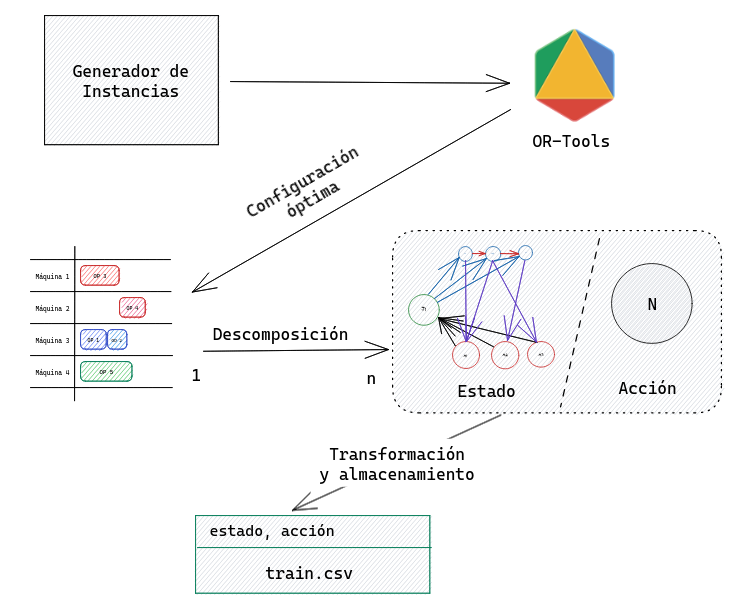
\includegraphics[scale=0.47]{generate_train.png}
    \caption{Pipeline para generar el train.csv}
    \label{fig:trainingpipeline}
\end{figure}

\subsubsection{Funcion de entrenamiento}
Una vez que se ha generado el dataset de entrenamiento, se puede proceder a entrenar el modelo.
Se va a definir una funcion train que recibe como parametros el modelo, el optimizador, el dataset
que hemos generado previamente y el tamaño del batch. Esta funcion se encarga de entrenar el modelo
y devolver el calculo del loss que se ha obtenido durante el entrenamiento.\medskip

\begin{lstlisting}
def train(model, optimizer, train_loader, batch_size):
    model.train()
    softmax = torch.nn.Softmax(dim=0)
    total_examples, total_loss = 0, 0

    for batch in train_loader:
        optimizer.zero_grad()
        action_prob = torch.Tensor([])
        result = model(batch)

        list_action_prob = []
        list_targets = []

        for i in range(batch["job"].batch[-1] + 1):
            action_probs = result[batch_index == i].T[0]
            action_prob = softmax(action_probs)
            list_action_prob.append(action_prob)
            list_targets.append(
                batch[("machine", "exec", "job")].y[batch_index == i]
            )

        loss = F.binary_cross_entropy(list_action_prob, list_targets)
        loss.backward()
        optimizer.step()

        total_examples += batch_size
        total_loss += float(loss) * batch_size

    return total_loss / total_examples 
\end{lstlisting}\medskip

Esta funcion es la responasable de efectuar el Imitation Learning, para ello carga en el
trainloader los grafos que habiamos generado previamente y se le pasa al modelo para que
realice la predicción. Una vez que se tiene la predicción, se calcula el loss y se compara
con la solución que ha tomado el experto para ese estado. Una de las particularidades que
tiene el modelo es que la predicción que devuelve se realiza sobre el tensor que represnta 
la relacion entre las operaciones y las maquinas, por lo que aunque aumente o disminuya 
el numero de operaciones o maquinas no sera necesario modificar el modelo, ya que este 
se adapta a diferentes dimensionalidades.

\subsubsection{Arquitectura del ensemble}
Una vez que se ha entrenado el modelo basico, se puede proceder a montar el ensemble.
Como se ha comentado anteriormente, el ensemble se va a componer de 3 modelos, cada uno
de ellos se va a ejecutar de forma independiente y se va a recuperar la solución que 
mejor desempeño haya tenido. A continuación se muestra la arquitectura del ensemble.

\begin{figure}[ht]
    \centering
    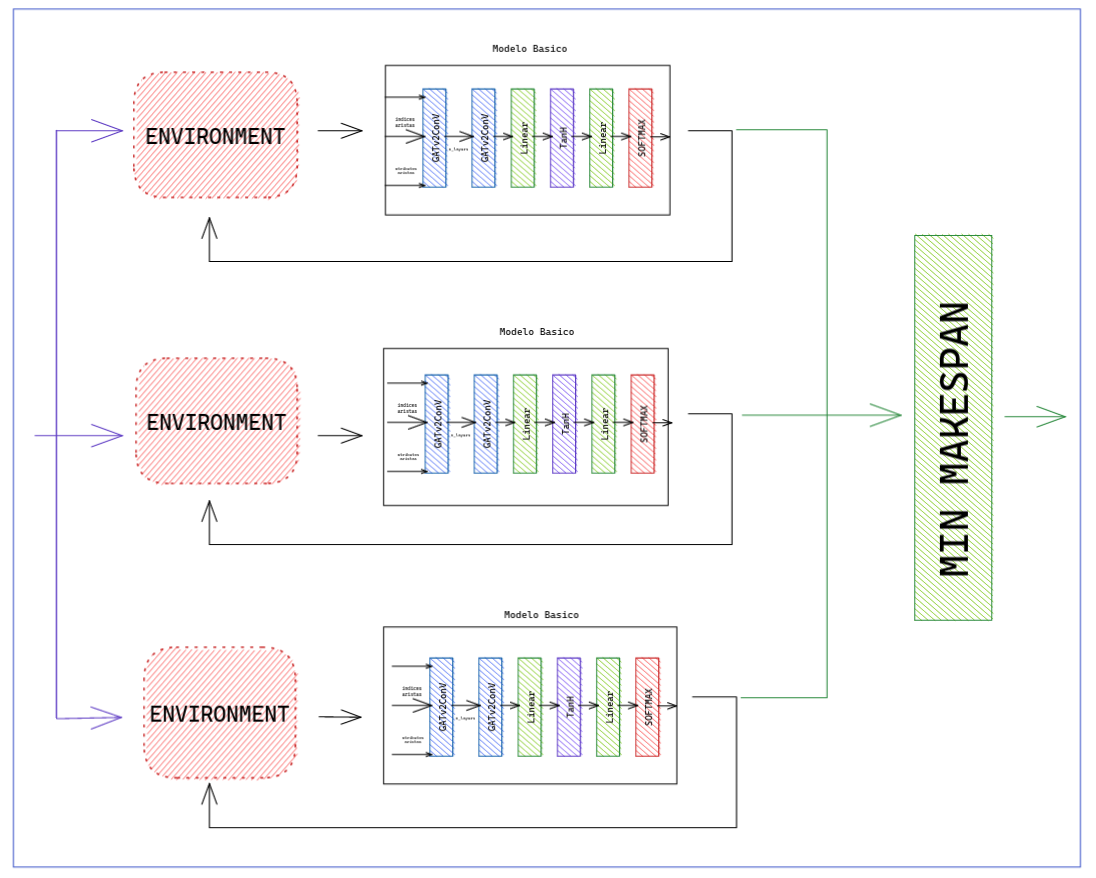
\includegraphics[scale=0.38]{ensemblearc.png}
    \caption{Arquitectura del ensemble}
    \label{fig:ensemblearc}
\end{figure} 

